\section{Method} \label{sec:method}
In this section, we first describe the dataset and the data preparation steps. Then we describe the experimental methods including the development and evaluation of predictive models.

\subsection{Dataset}\label{sec:dataset}
One-hundred seventy-eight ICU patient cases with a diagnosis of either acute kidney failure (AKF; ICD-9 584.9 or 584.5; 93 cases) or acute respiratory failure (ARF; ICD-9 518.81; 85 cases) were selected randomly from patients who were admitted between June 2010 and May 2012 to an ICU at the University of Pittsburgh Medical Center. Eleven critical care medicine physicians reviewed the patient cases in the LEMR system and for each patient indicated which patient information was relevant to the task of pre-rounding in the ICU.

The dataset consists of two sets of variables including the predictor variables (or predictors) and target variables (or targets) that we now describe in detail. Predictor variables include demographics, admitting diagnosis, vital signs, ventilator settings, input and output measurements, laboratory test results, and medication administration data. A few variables such as demographics and admitting diagnosis are static, that is, their values do not change during the ICU stay, while the remaining variables, which constitute the majority of the predictors, are temporal and have multiple values during the ICU stay. For example, age (in years) is a static predictor variable while blood urea nitrogen (BUN) is a temporal predictor variable as it is usually measured multiple times during an ICU stay.

Target variables include any data in the EMR, such as vital signs, ventilator settings, input and output measurements, laboratory test results, and medication administration data that a physician may annotate as relevant for the task of pre-rounding. A target variable can take either \textit{relevant} or \textit{not relevant} values. As an example, for a patient with AKF, BUN = \textit{relevant} denotes that BUN was measured for the patient and was sought, found, and annotated by a physician as relevant. If BUN was measured for the patient but was not sought by a physician, then the target is denoted as BUN = \textit{not relevant}. A target variable may be missing too; for example, when BUN is not measured for the patient, it would not be available for a physician to seek and find. We developed a predictive model for each target variable such as BUN that predicts whether it is relevant in a particular patient. To develop a BUN model, we used all predictor variables described in the previous paragraph and used only data in which the BUN target was not missing. 

The difference between predictor and target variables is in the values they take; i.e., a target variable takes values of either \textit{relevant} or \textit{not relevant}, whereas a predictor variable’s values are the measured values that are recorded in the EMR. For example, when BUN is a predictor, it takes numeric values in milligrams per deciliter (mg/dL) unit\footnote{Note that BUN may have been measured multiple times for a patient case and therefore, take several numeric values. We summarize these values as a fixed-length vector as described in the Data preparation section.}, whereas as a target variable, it takes a value of either relevant or not relevant. Consequently, a model for predicting whether or not BUN is relevant may contain numeric values for BUN as a predictor variable.

\subsection{Data preparation}\label{sec:data_prepration}
We transformed the dataset into a representation that is amenable to the application of machine learning methods. In particular, for each temporal predictor variable we generated between 4 to 36 features (feature expansion in Figure~\ref{fig:1}).

The number of features for a temporal predictor was based on (1) the data domain of the predictor variable (e.g., medication administration or laboratory result) and (2) the type of the predictor variable (e.g., nominal or continuous). For example, for each medication variable we generated four features including an indicator of whether the drug is currently prescribed, the time elapsed between first administration and the current time, the time elapsed between the most recent administration and the current time, and the dose at the most recent administration. For each laboratory test result, vital sign, and ventilator setting, we generated up to 36 features including an indicator of whether the event or measurement ever occurred, the value of the most recent measurement, the highest value, the lowest value, the slope between the two most recent values, and 30 other features. More details on the feature expansion are given in \cite{king2018development}.

The dataset consisted of 178 patient cases and 1,864 raw predictor variables. Feature expansion resulted in a total of 30,770 features. Since the dimensionality of the data was high, we reduced the number of features (feature reduction in Figure~\ref{fig:1}) by removing those features where the values were missing in every patient case, had the same value for every case (i.e., had zero variance), or the values were duplicates of another variable. Feature reduction resulted in a total of 6,935 features.

We selected as target variables 73 EMR data items that had been annotated as relevant (positive) in 9 or more patient cases. Table~\ref{tab:s1} in Appendix \ref{sec:app_C} contains the list of target variables along with the number of cases in which each target variable was relevant, as well as the number of cases where the target variable was available for selection (i.e., the value was not missing). 

\begin{figure}[!h]
    \centering
    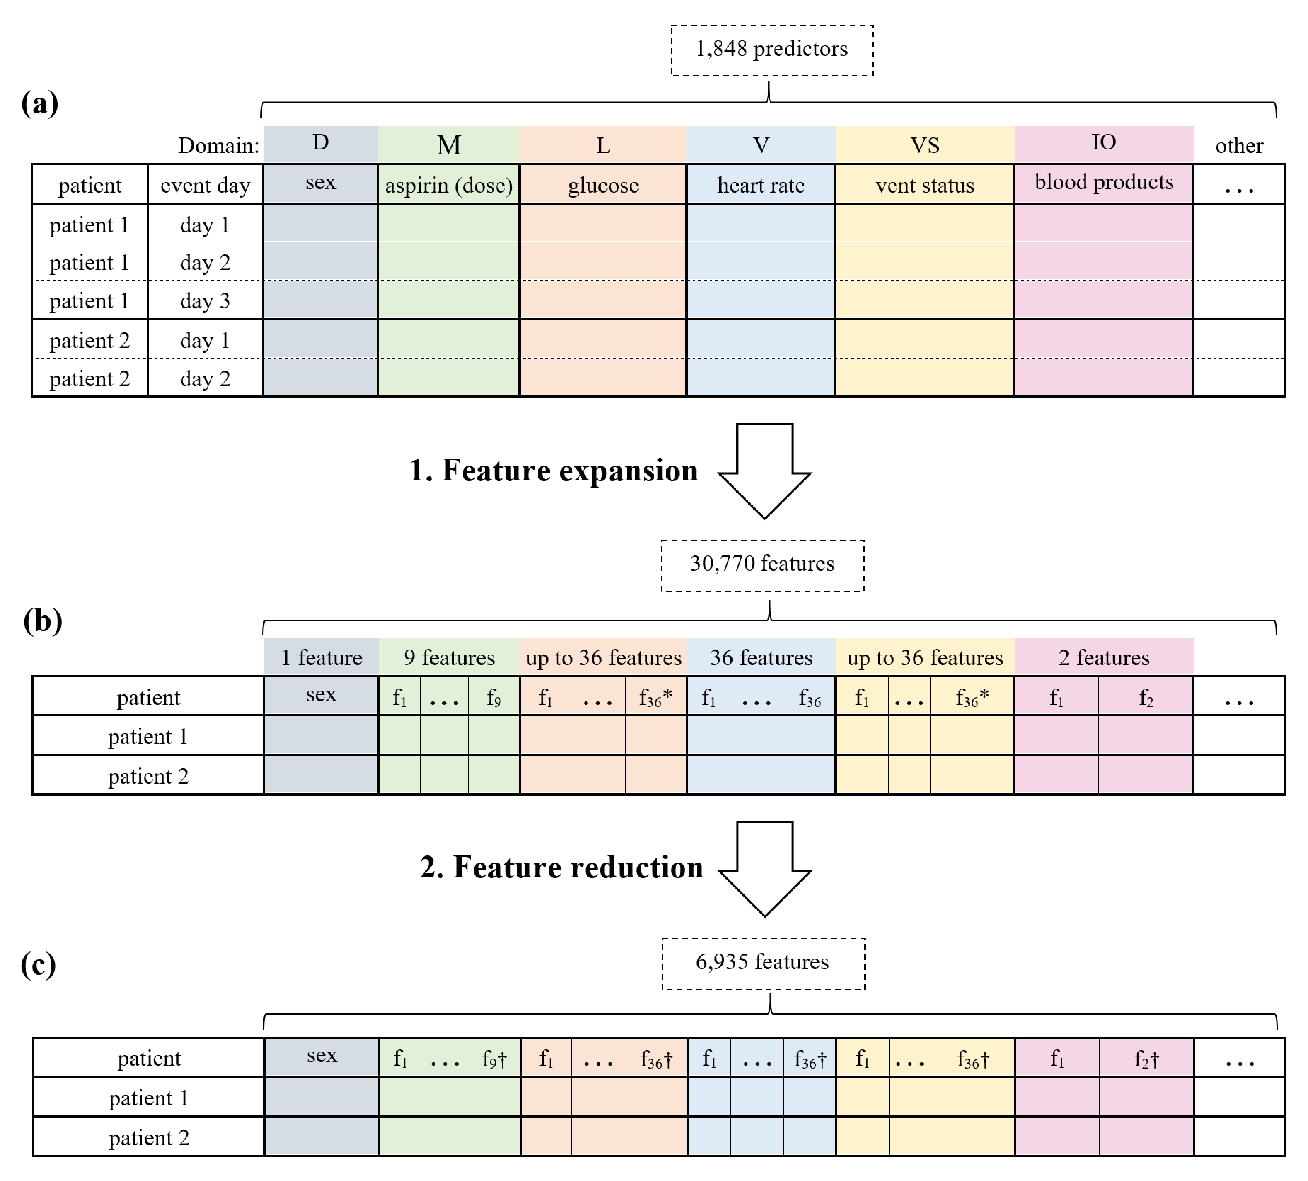
\includegraphics[width=\textwidth]{./pictures/Figure1}
    \caption{
    Steps in preparing the predictor variables. \textbf{(a)} presents the predictor variables for two example patients as measurements with one row per day. The colors represent data domains; D=demographics, M=medication administrations, L=laboratory test results, V=vital signs, VS=ventilator settings, IO=input/output, and other=other domains. \textbf{(b)} shows the result of expanding the temporal predictor variables (total = 1,848) to features (total = 30,770). This step flattens the data so that a patient that is represented by multiple rows is now represented by a single row. * denotes that the number of expanded predictors differs depending on the predictor value type (e.g., nominal or continuous). \textbf{(c)} shows the features after feature reduction, in which the number of features is reduced to 6,935s. † indicates that the number of features may be different for each variable in the domain.
    }\label{fig:1}
\end{figure}

\subsection{Experimental methods}\label{sec:exp_methods}
\subsubsection{Predictive models}
An HLR model is a generalization of a standard logistic regression model in which the data is clustered into groups and the model intercept and coefficients can vary by group \cite{gelman2006data}. Figure~\ref{fig:2} shows the structure of a 2-level HLR model in which the LEMR data is clustered into groups of patient cases reviewed by each physician. Parameters at the lower level represent the physician-level models for the 11 physician reviewers, and parameters at the upper level represent the model for the entire population of physician reviewers (i.e., population-level model). For a more detailed description of HLR models see Appendix~\ref{sec:app}.

\begin{figure}[!h]
    \centering
    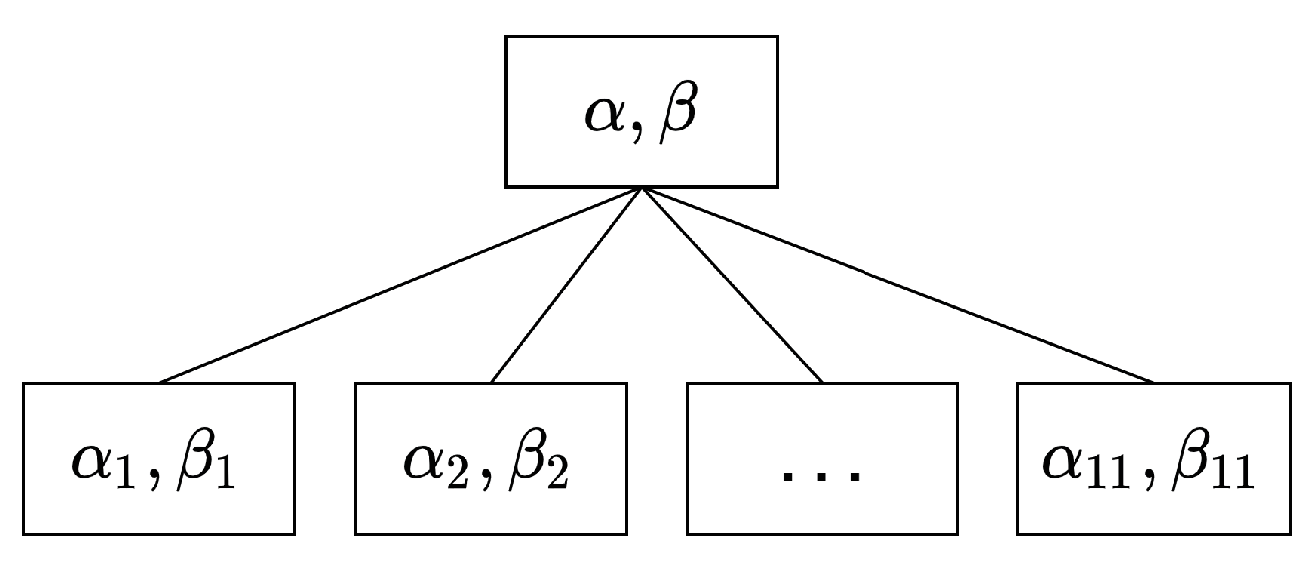
\includegraphics[width=0.6\textwidth]{./pictures/Figure2}
    \caption{
    A 2-level HLR model for LEMR data. The lower level represents physician-level intercepts ($\alpha_i$) and coefficients ($\beta_i$) where $i=1,...,11$ denotes the physician identifier. The upper level represents the intercept and coefficients ($\alpha$, $\beta$) for the population-level model.}\label{fig:2}
\end{figure}

We developed HLR predictive models for each of the selected 73 targets. Each predictive model of a target variable is formulated as a binary classification problem where the model learns to identify cases in which the target variable is relevant. To investigate the utility of HLR over non-hierarchical models, we used LR as baseline models in which the physician identifier was included as an indicator variable. We implemented the HLR models using the brms package \cite{Burkner2017} in R, which uses No-U-Turn Sampler (NUTS) (as an extension of the Hamiltonian Monte Carlo algorithm) to estimate the posterior distribution of model parameters. In our experiments, we set the NUTS sampler to use 4 Markov chains; each chain included 400 iterations of sampling where the first 200 were used to calibrate the sampler. A total of $4 \times 200 = 800$ posterior samples for each HLR model parameter were obtained. LR models were implemented using the glmnet package in R \cite{Friedman2010}.

\subsubsection{Cross validation}\label{sec:crossvalidation}
Each model was trained and evaluated independently in a stratified 10-fold cross validation setting. At each iteration of the cross validation, the patient cases were randomly split into a training set (9 folds) and a test set (1 fold), while preserving the original distribution of the target variable. Hyperparameter tuning and data preprocessing such as imputing missing values and feature selection were performed during cross validation. More details are described in Appendix~\ref{sec:app_B}.

\subsubsection{Performance measures}\label{sec:measures}
We measured the predictive performance of each model with the area under the receiver operating characteristic (ROC) curve (AUROC), area under the precision-recall curve (AUPRC), and expected calibration error (ECE) \cite{Naeini2015}. AUROC is a measure of model discrimination and varies from 0.5 and 1, where 0.5 denotes an uninformative model and 1 represents perfect discrimination. AUPRC summarizes the precision-recall curve where precision (or positive predictive value) and recall (or sensitivity) values at different thresholds are plotted as a curve. The AUPRC varies from 0 to 1 is and is commonly used in binary classification problems when the data is imbalanced (i.e., when cases with one label are more prevalent than cases with the other label).

ECE is a measure of model calibration. In a perfectly calibrated model, outcomes with predicted probability  correspond to a fraction  of positive cases in the data. ECE is derived from the probability calibration curve \cite{degroot1983comparison} where the sorted predicted probabilities are partitioned into  bins; in each bin $i$, calibration error is defined as the absolute difference between the mean of predicted probabilities ($p_i$) and the fraction of positive outcomes ($o_i$). ECE is the weighted average of the calibration errors over all  bins:

\begin{equation}\label{eq:1}
   \text{ECE} = \sum_{i=1}^{k}{w_i |p_i - o_i|} 
\end{equation}
where $w_i$  denotes the fraction of cases that fall into bin $i$. Lower ECE denotes a better calibrated model.


